\documentclass[14pt,final]{report}
% \usepackage[english,russian]{babel}

% \RequirePackage{polyglossia}
% \setotherlanguage{english}
% \setdefaultlanguage{russian}

\RequirePackage[times,firacode,a4paper,microtyping,732,smalltitles,listbib]{subook}
% \RequirePackage[times,firacode,a4paper,microtyping,handbook,smalltitles,listbib]{subook}
\RequirePackage{tabularx}
% \RequirePackage{grphicx}
\graphicspath{{pics/}}

\usepackage{showframe}

% pygmetize
\RequirePackage{minted}
\usemintedstyle{tango} % bw

% \setmainfont{Times New Roman}

\begin{document}
\thispagestyle{empty}
\begin{center}
МИНИСТЕРСТВО ОБРАЗОВАНИЯ И НАУКИ РОССИЙСКОЙ ФЕДЕРАЦИИ

Федеральное государственное бюджетное образовательное учреждение высшего образования

«ИРКУТСКИЙ  ГОСУДАРСТВЕННЫЙ УНИВЕРСИТЕТ»\\
(ФГБОУ ВО «ИГУ»)
\end{center}
\vfill % \vfil \vfill \vfilll

\noindent\begin{tabularx}{\textwidth} {
  >{\raggedright\arraybackslash}X
  >{\raggedright\arraybackslash}X }
Институт математики и информационных технологий
&
Кафедра теории вероятностей и дискретной математики
\end{tabularx}

\vfill
\begin{center}
  \textbf{ОТЧЕТ}
\vspace{1em}

о курсовой работе по курсу <<Разработка WEB-приложений>>

{\bf Проектирование системы учета радиодеталей}

\end{center}
\vfill

\noindent\begin{tabularx}{\textwidth} {
  >{\raggedright\arraybackslash}X
  >{\raggedright}X }
&

Студентки 4 курса группы 2361\\
Фамилия Имя Отчество\\
Направление\;: 02.03.03~--~Математическое обеспечение и администрирование информационных систем\\[2em]

Руководитель:\\
канд.~техн.~наук доцент\\
Иванов Иван Иванович\\[2em]

Курсовая работа защищена с оценкой\\[1em] \underline{\hspace{3cm}}
\end{tabularx}
\vfill
\begin{center}
  Иркутск -- 2021
\end{center}
\clearpage

\tableofcontents

\chapter*{ВВЕДЕНИЕ}
% TODO: Add contents line
\label{chap:intro}

\chapter{Теоретические основы ....}

Согласно \cite{bratko90}

.... база данных (БД) .....

\chapter{Реализация ....}

\section{Скрипт порождения структуры базы данных}
\label{sec:struct-bd}

Начало абзаца


\begin{figure}[htbp]
\begin{center}
\begin{minted}[fontsize=\normalsize]{sql}
CREATE TABLE Persons (
    PersonID int,
    LastName varchar(255),
    FirstName varchar(255),
    Address varchar(255),
    City varchar(255)
);
\end{minted}
\end{center}
\caption{Скрипт SQL для создания таблицы Persons}\label{fig:crate-table}
\end{figure}


\begin{listing}[htbp]
\begin{center}

{\footnotesize
\begin{verbatim}
CREATE TABLE Persons (
    PersonID int,
    LastName varchar(255),
    FirstName varchar(255),
    Address varchar(255),
    City varchar(255)
);
\end{verbatim}}

\end{center}
\caption{Скрипт SQL для создания таблицы Persons}\label{fig:crate-table}
\end{listing}

\chapter{Тестирование ....}

Разработан набор тестов структуры БД (см.~\ref{sec:struct-bd} на стр.~\pageref{sec:struct-bd}).   Загрузка скрипта базы данных осуществляется при помощи команды \texttt{mysql}.  Дамп существующей БД выполняется командой \verb|mysql-dump|.

\begin{figure}[hbtp]
  \centering
  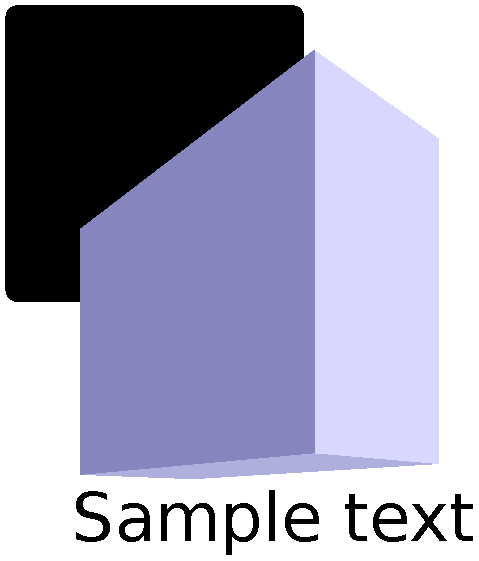
\includegraphics[width=0.3\linewidth]{fig1.pdf}
  \caption{Пример работы программы}
  \label{fig:prog-ex}
\end{figure}


\begin{equation}
  \label{eq:f1}
  E=mc^2
\end{equation}

\noindent{}где, $m$ -- это масса, $c$ -- скорость света в вакууме, \ldots

Новый абзац. Рассмотрим формулу (\ref{eq:f1}).


\chapter*{ЗАКЛЮЧЕНИЕ}



\begin{thebibliography}{99}
\bibitem{bratko90} И.~Братко. Язык программирования Пролог для искусственного интеллекта. М\;:~Наука. 1990. 310~c.
\end{thebibliography}

\appendix

\chapter{Исходный код программ}
\chapter{Документация разработчика}

\end{document}




%%% Local Variables:
%%% mode: latex
%%% TeX-master: t
%%% End:
